\chapter{Probing the ultra-dense matter}
\chapterimage[width=15cm]{wordcloud/chap4b.png}

The main motivation for this thesis was to set constraints for equation of state of the ultra-dense matter inside neutron stars.
Instead of starting from the nuclear physics that works on the smallest scales, we use astrophysical observations to study large-scale ``global'' aspects of neutron stars.
It is then possible to make a step back to the nuclear physics because the size of a compact star is strongly coupled to the composition of its core.

Looking from the astrophysical point of view, it is the size of the neutron star that will define many of its observable features.
One of the most important characteristics is the compactness of the object that will then define the exact shape of the spacetime surrounding it.
The strongly curved spacetime, in turn, influences many of the phenomena occurring in the close vicinity of the star and will also leave its distinct imprints on the observations.

The physical phenomena behind the observable features on the other hand, are often highly energetic, otherwise they would not be seen by distant observers, such as us.
It is these highly energetic physical processes that will then render the neutron stars visible to us, and that at the same time carry a plethora of information from the surroundings of where they originated from.
This gives birth to a beautiful connection where the delicate and unattainable nuclear physics of the ultra-dense matter is coupled to vigorous astrophysical phenomena that we can observe.
The caveat here is that the astrophysical processes are often messy and poorly understood.
Hence, a thorough understanding of both, the nature of the observed phenomena and how it exactly couples to the nuclear physics, is needed.

In this thesis, we will focus on extracting the information from the X-ray bursts.
In theory, this method of using the X-ray bursts to probe the neutron star interiors is robust as we can theoretically model the characteristics of the emerging radiation and these models can be applied to describe the data that we see. 
In practice, however, caution is needed when applying the models as the environment and the astrophysics near the neutron star play a huge role.


In this final chapter, we will lay out the basics of how by observing the burst cooling it is possible to set constraints on the size of the emitting area, and in the end, the radius of the neutron star.
We will also summarize the content of the articles in this thesis\refedel{,} and discuss our work where we try to understand not only the complex role of the astrophysical surroundings but in the end, the composition of the core.


\section{Measuring the sizes of the bursting sources}

Even though the bursts characteristics change from one burst to another as we saw in \sect{sect:bursts}, the cooling appears to obey some common trends.
This means that as long as we have some kind of \refedel{an} energy injection deep below the neutron star's atmosphere, the energy will radiate out and the uppermost layers of the star will then shape it into a similar cooling curve, independent of the actual details of the injection.
If we are then able to model the atmosphere and the processes therein, we can use the bursts as probes for the neutron star interiors.
Note, however, that not every burst is powerful enough to be of practical use.
As we shall see, we additionally require that the bursts reach the Eddington limit, which in practice means using the PRE-bursts only.

%Let us, however, momentarily push these complications aside and assume that when observing the X-rays from the bursts, the radiation detected is dominated by the burst emission from the neutron star surface.
%This allows us to put interesting limits on the size and the mass of the emitting source.
To begin, let us define three different families of quantities: 
observed quantities ($\mathrm{obs}$), theoretical quantities predicted by our model at infinity ($\infty$), and the same theoretical model quantities in the local frame of the star ($*$).
This is done, because general relativistic effects change the local physical quantities as they travel from the star to a distant observer.\cite[see e.g.,][]{Lewin93}
More specifically, we can connect the temperatures $T$, radii $R$, and luminosities $L$ as
\be\label{eq:Rz}
R_{\infty} = R_* (1+z),
\ee
\be\label{eq:Tz}
T_{\infty} = \frac{T_*}{1+z},
\ee
\be\label{eq:Lz}
L_{\infty}= \frac{L_*}{(1+z)^2},
\ee
where $(1+z$) is the redshift factor that is related to the previously defined compactness $u = 2GM/Rc^2$ as
\be
1+z = (1 - u)^{-1/2}.
\ee
From the observations, we see that the detected burst spectra are reasonably well described by the Planck function (blackbody) as
\be
F_{E, \mathrm{obs}} \approx \pi B_E(T_{\mathrm{obs}}) K_{\mathrm{obs}},
\ee
where $B_E(T_{\mathrm{ obs}})$ is a blackbody function with a measured temperature $T_{\mathrm{obs}}$ and normalization $K_{\mathrm{obs}}$, together with $E$ which is \refe{the photon} energy that we observe at.
The normalization for an \refedel{circular} object at a distance $D$ in the sky is
\be\label{eq:Robs}
K_{\mathrm{obs}} = \frac{R_{\mathrm{obs}}^2}{D^2}.
\ee
Observed bolometric flux is then
\be
F_{\mathrm{obs}} = \int_0^{\infty}F_{E, \mathrm{obs}} dE = \sigmaSB T_{\mathrm{obs}}^4 \frac{R_{\mathrm{obs}}^2}{D^2}.
\ee

\begin{figure}[t!]
\centering
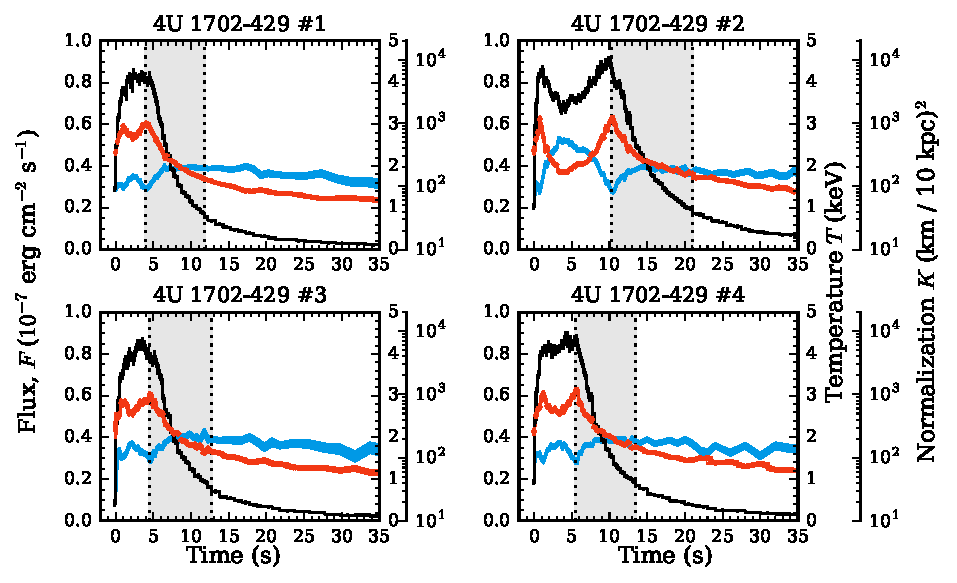
\includegraphics[width=16cm]{figs/constraints/bursts.pdf}
\caption{\label{fig:bursts}
Examples of bolometric flux, temperature and blackbody normalization evolution during the hard-state PRE bursts. 
The black line shows the estimated bolometric flux (left-hand vertical axis) in units of $10^{-7} \unitspace\erg\unitspace\cm^{-2}\unitspace\mathrm{s}^{-1}$.
The blue ribbon shows the blackbody normalization (outer right-hand vertical axis) in $(\km/10\unitspace\mathrm{kpc})^2$.  
The red ribbon show\refe{s} the blackbody temperature (inner right-hand vertical axis) in keV. 
Highlighted gray area marks a typical region of the cooling tail used in the fitting procedures.
}
\end{figure}

Some examples of Planck function fit results for X-ray bursts are shown in \fig{fig:bursts}.
Here the time-dependent spectral fits are shown for one particular source, 4U 1702$-$429.\cite[see][for more detailed description of the data]{NSK16, NMS17}
All of the bursts shown here are exhibiting the photospheric radius expansion, that can be seen from the characteristic dip in the normalization and of the simultaneous maximum in the temperature.\cite[see e.g.,][]{GMH08}
The flux corresponding to the exact moment when the photosphere collapses back to the neutron star's surface is dubbed the touchdown flux, and it is visualized by the first vertical dotted line in the figures.


From the atmosphere models of neutron stars, we obtain a similar result.
The local detailed model spectra \refe{are} well approximated by a so-called diluted blackbody model given as
\be
F_{E,*} \approx \pi w B_E(\fc \Teffs),
\ee
where $w$ is the dilution factor, $\fc$ is the color-correction factor, and $\Teffs$ is the effective temperature of the atmosphere.
This allows us to connect the observed values to the theoretical model values by first redshifting these quantities to infinity.
From \eq{eq:Tz}\ we simply obtain that the temperature of the model as seen by a distant observer must be
\be
\fc \Teffi = \fc \frac{\Teffs}{1+z}.
\ee
Similarly, the area of the star on the sky must be related not to $R_*$ but to $R_{\infty}$ as given by \eq{eq:Rz}
\be\label{eq:Rmod}
w \frac{R_{\infty}^2}{D^2}= w \frac{R_*^2 (1+z)^2 }{D^2}.
\ee
The latter \eq{eq:Rmod}\ gives immediate constraints for the radius as it can be equated with the observed size \eqref{eq:Robs}\ as\cite{Penninx89, vParadijs90}
\be
%\frac{R_{\mathrm{obs}}^2}{D^2} =  w \frac{R_{\infty}^2}{D^2}= w \frac{R_*^2 (1+z)^2 }{D^2}.
R_{\mathrm{obs}}^2 =  w R_{\infty}^2= w R_*^2 (1+z)^2.
\ee

Additional constraints can be obtained by measuring the Eddington limit of the source.
As we have seen, there exists a flux for which the radiation forces equal to the gravitational forces (see \sect{sect:Eddington}), given as 
\be
F_{\mathrm{Edd},*} = \frac{G M c}{\kappa_{\mathrm{T}} R_*^2} (1+z),
\ee
where $\kappa_{\mathrm{T}} = 0.2(1+X)\unitspace\cm^2\unitspace\g^{-1}$ is the Thomson electron scattering opacity and $X$ is the hydrogen mass fraction.
One should note here that even though we use the Thomson electron scattering opacity in the notation, one is not restricted to assuming this.
It is, for example, possible to take the Klein-Nishina reduction in the cross-section into account which formally allows for super-Eddington fluxes.\cite{SPW12}
In reality the Eddington limit is, of course, still respected.
Using this characteristic flux we can also define the Eddington luminosity $L_{\mathrm{Edd},*}$ and the corresponding Eddington temperature $T_{\mathrm{Edd},*}$ as
\be
L_{\mathrm{Edd},*} =  4\pi R_*^2 F_{\mathrm{Edd},*} = 4\pi R_*^2 \sigmaSB T_{\mathrm{Edd},*}^4.
\ee
These are again quantities defined near the star whereas what one observes at infinity are given by
\be
L_{\mathrm{Edd},\infty} = \frac{ L_{\mathrm{Edd},*} }{(1+z)^2},
\ee
\be
F_{\mathrm{Edd},\infty} = \frac{L_{\mathrm{Edd},\infty}}{4\pi D^2} = \frac{G M c}{\kappa_{\mathrm{T}} D^2} \frac{1}{1+z},
\ee
and
\be
T_{\mathrm{Edd},\infty} = \frac{T_{\mathrm{Edd},*}}{1+z}.
\ee

As the simplest case, we can obtain additional constraints for the radius and mass by just measuring the $F_{\mathrm{Edd},\infty}$ somehow.
This can be done, for example, by equating it with the touchdown flux obtained from the time-dependent burst spectra.
This is the basis of the so-called ``touchdown method''.\cite{Ebi87, vParadijs90, Ozel06, Ozel16}

A more sophisticated version of this is the so-called ``cooling tail method''.\cite{SPRW11, PNK14}
Here we can compute the varying color-correction factor $f_{\mathrm{c}}$ from the atmosphere models as a function of $\ell \equiv L_*/L_{\mathrm{Edd,*}}$.
In this case, the dilution factor was obtained from the approximative relation $f_{\mathrm{c}} \approx w^{-4}$.
The color-correction factor can then be related to multiple $K_{\mathrm{obs}}$ measurements, each representing  one time snapshot from the cooling tail.
As the time passes and the surface cools down, the flux decreases.
This allows us to compare the model dependency of $\ell$ vs. $f_{\mathrm{c}}$ to the observations of $F_{\mathrm{obs}} / F_{\mathrm{Edd}, \infty}$ vs. $K_{\mathrm{obs}}^{-1/4}$.
Hence, extra information from the observations is used because not only are the individual color-correction factor values compared against the model but also their full dynamic evolution as a function of flux is taken into account.
The fitting procedure is two dimensional in this case as we fit $F_{\mathrm{Edd},\infty}$ and $R_{\infty}^2/D^2$ as free parameters simultaneously.
Interestingly, the combination of these two fit parameters then yield a distance-independent quantity, physically corresponding to the Eddington temperature of the source at infinity, given as
\be
T_{\mathrm{Edd},\infty} 
%= 9.81 
= \Ten{1.14}{8}
\left( \frac{F_{\mathrm{Edd},\infty}}{10^{-7}\unitspace\erg\cm^{-2}\unitspace\mathrm{s}^{-1}} \right)^{1/4}
\left( \frac{(\km/10\unitspace\mathrm{kpc})^2}{R_{\infty}^2/D^2}  \right)^{1/4} 
\Kelvin.
%\unitspace\mathrm{keV}.
\ee
This corresponds to a parametric relation for the $M$ and $R$ via the compactness $u$, given as
\begin{align}\begin{split}
R &= \frac{c^3 u(1-u)^{3/2}}{2\kappa_{\mathrm{T}} \sigmaSB T_{\mathrm{Edd},\infty}^4} 
\approx 1188 \frac{u(1-u)^{3/2}}{(1+X) T_{\mathrm{Edd},\infty, 7}^4} \km, \\
M &\approx u \frac{R}{2.95\km} \Msun, \\
\end{split}\end{align}
where $T_{\mathrm{Edd},\infty,7} = T_{\mathrm{Edd}, \infty} / 10^7 \Kelvin$.
Later on, another variant of this method was introduced, called ``direct cooling tail method'' where the assumption of $f \approx w^{-4}$ was relaxed, i.e., both $f_{\mathrm{c}}$ and $w$ are considered, and the fitting is done directly via the $M$, $R$ and $D$ parameters.\cite{NSK16, SPN17} 


The usage of these methods on X-ray burst data span almost three decades of scientific work as of now.
Starting from the early work in the late 80s they have since improved and been applied to various sources to estimate the radius and mass.
Latest in the family\refedel{,} is the method of fitting the observed data directly with the atmosphere models.\cite{NMS17}
Although computationally more demanding exercise, it allows us to finally extract every piece of information possible from the data.
This is based on the additional model dependency on the surface gravity, composition, and detailed spectral shape that slightly deviates from the Planck function.


The big caveat here for any of the aforementioned methods is the surroundings.
We have seen that the astrophysical environment of neutron stars can be very active and lively.
In the general picture, we have the accretion as an energy source and the disk to dissipate this energy.
The disk is, however, not a simple geometrically thin steady layer but can have complex inner flow.
On the other hand, if the disk does extend all the way down to the star, an additional complication originates from the boundary or spreading layer that not only can cover the star but also radiate on its own.
These are some of the complications that we face when trying to analyze our neutron star observations, as after all when trying to constrain the mass and radius of the star we must make sure that it is actually the star that we are looking at.


\section{Scientific summary of the results}

In this thesis, we have focused on constraining the equation of state of the cool ultra-dense matter inside neutron stars with astrophysical measurements.
The main results are two-folded as we have both
\begin{itemize}
\item improved our understanding of ultra-dense matter and have been able to put stringent constraints on the equation of state of the neutron star interiors, and
\item progressed our understanding of neutron star environments and astrophysics of X-ray burst.
\end{itemize}
To be able to do this, we had to develop our observational and statistical methods, do theoretical research in order to understand the astrophysical scenarios better, develop and improve our physical models, and finally apply these new methods and information to real-world observations.
Because of this, the results and work in this thesis can be divided into three categories that we now discuss in more detail. 
In short, these include \textit{1}) theoretical work on the models, \textit{2}) understanding the astrophysical environment better, and \textit{3}) applying the models and the new insights to astronomical observations.


\subsection{Modeling of neutron star atmospheres and emergent radiation}

Computing hot neutron star atmosphere models for the X-ray bursters is of paramount importance for obtaining the mass and radius measurements from the burst observations.
More specifically, we are interested in the color correction factor $f_{\mathrm{c}}$ and the dilution factor $w$, in order to compare our knowledge to observations.
Previous models for hot atmospheres have all assumed simple hydrogen, helium, or solar composition for the plasma.
In some cases, however, the burning ashes may rise from the burning depths up to the photosphere, leading to the appearance of the metal absorption edges in the spectra.
These effects may have a substantial impact on the color correction factor and the dilution factor $w$.
In paper I, we have developed a new atmosphere modeling code to compute the emergent spectra for a composition consisting of any atomic species.
We find that the metals may change $f_{\mathrm{c}}$ by up to about 40\%.
The presented models also made possible to determine the NS mass and radii more accurately for cases when we do see signs of burning ashes, and provided a new tool to probe the nuclear burning mechanisms in X-ray bursts.

The radiative process that we consider all occur at or near the neutron star.
Because of this, many general relativistic effects play an important role in shaping the observations.
In paper II, a theoretical framework for emission originating from rapidly rotating oblate compact objects was described in detail.
In order to solve the geodesic equation, a new split Hamilton-Jacobi formalism was constructed for a metric that is expanded up to second order in rotation and hence includes effects of light bending, frame-dragging, and quadrupole corrections for the photon trajectories.
We also gave detailed descriptions of the numerical algorithms used and provide an open\refe{-}source implementation of the numerical framework called \textsc{bender}.
As an application, we study spectral line profiles from rapidly rotating oblate neutron stars. 
The Full Width at Tenth Maximum and Full Width at Half Maximum for the so-called smearing kernels are also reported for all of the possible viewing angles.
These can be then used to quantitatively estimate the effects of rotational smearing on the observed spectra.
%We also calculated pulse profiles and observer skymaps of emission from hot spots on rapidly rotatingaccreting millisecond pulsars.
%These allowed us to quantify the strength of the pulse fractions one expects to observe from typical fastly spinning millisecond pulsars.


\subsection{Understanding the astrophysical environments of X-ray bursts}
As we have seen, the neutron star environment is an important factor that needs to be understood before reliable mass and radius estimates can be obtained from X-ray burst observations.
In paper III, we study the effects of accretion for one particular source, LMXB system 4U 1608$-$52.
We found a strong dependence of the burst properties on the flux and spectral hardness of the persistent emission before burst. 
Bursts occurring during the low accretion rate (hard) state exhibit evolution of the blackbody normalization consistent with the theoretical predictions of neutron star atmosphere models. 
However, bursts occurring during the high accretion rate (soft) state show roughly constant normalization, which is inconsistent with models and therefore these bursts cannot be easily used to determine neutron star parameters. 

In the next paper IV, we continue our analysis further by studying 246 X-ray bursts in total, from 11 different LMXB systems.
Again, we found a dependence between the persistent spectral properties and the time evolution of the blackbody normalization during the bursts. 
The neutron star atmosphere model predictions agree with the observations for most bursts occurring in hard, low-luminosity, spectral states, but rarely during soft, high-luminosity, states. 
We attributed the observed phenomena to the accretion flow, which can influence the cooling of the neutron star especially during the soft state when the accretion rate is high.
The results had the important implication that only the bursts occurring in the hard, low-luminosity spectral states could be reliably used for mass and radius determination.





\subsection{Constraining the mass and radius of neutron stars}

By now applying the atmosphere model results to the X-ray burst data, we can try to set constraints for the size of the emitting source.
However, here it is crucial to take into account also the accretion rate, i.e., consider bursts that occur during the hard-state only.
In paper V we did this analysis for three different LMXB systems: 4U 1702$-$429, 4U 1724$-$307, and SAX J1810.8$-$260. 
This allows us to set constraints for the masses, radii, compositions, and distances of the neutron stars in those systems.
We then obtained a parameterized equation of state by comparing the resulting neutron star structures to the radius and mass measurements we had.
%This was done by solving the TOV-equations (see \sect{sect:TOV}) and then using Monte Carlo algorithm within a Bayesian framework to obtain constraints for the underlying equation of state parameters.
This was done by solving the TOV-equations and then using Monte Carlo algorithm within a Bayesian framework to obtain constraints for the underlying equation of state parameters.
This allows us to set limits on various nuclear parameters and to constrain an empirical pressure-density relationship for the dense matter. 
Our predicted equation of state leads to a neutron star radius between $10.5$ to $12.8\km$ for a mass of $1.4\Msun$.  


The bursts that we considered in the aforementioned publication, were constrained to have an atmosphere consisting of almost fully of hydrogen and helium.
This is always not the case as explosive nuclear burning can fuse H and He into heavier elements too.
In paper VI, we presented our analysis of one particularly interesting long burst observed from the neutron star in LMXB system HETE J1900.1$-$2455. 
New atmosphere model fits to \refe{these} bursts indicated that sometimes the photosphere can consist entirely of metals, i.e., nuclear burning ashes.
These heavy metals like iron and nickel were detected already early on during the burst, which makes it possible that a radiatively driven wind might eject some of these ashes also into the interstellar space.
Hence, neutron star X-ray bursts might be one possible source of interstellar pollution.

Most previous works on X-ray bursts have used the Planck functions as a proxy to simplify the model vs. data comparison.
In paper VII, we, for the first time, fitted neutron star atmosphere models directly to the observed spectra.
This was done using a new nested hierarchical Bayesian model that allowed us to set new limits on mass, radius, composition, and distance of the neutron star in 4U~1702$-$429. 
We then find a radius of $R = 12.4\pm 0.4~\mathrm{km}$, gravitational mass $M=1.9\pm 0.3\Msun$, distance $5.1 < D/\mathrm{kpc} < 6.2$, and hydrogen mass fraction $X < 0.09$ with a $68\%$ confidence for this source.




\section{The author's contribution to the publications} 

\subsubsection*{Paper I.: Models of neutron star atmospheres enriched with nuclear burning ashes}
The author contributed to the main idea of the paper, independently redesigned the neutron star atmosphere code used for the calculations, and implemented new physical processes to this numerical framework. 
The author also prepared most of the manuscript together with J. Kajava.


\subsubsection*{Paper II.: Radiation from rapidly rotating oblate neutron stars}
The author proposed the idea of applying the split-Hamilton method to the ray tracing problem and designed the numerical code for the calculations. 
The theoretical framework and the related formulae were derived together with P. Pihajoki. 
The manuscript was also prepared together with P. Pihajoki.


\subsubsection*{Paper III.: The effect of accretion on the measurement of neutron star mass and radius in the low-mass X-ray binary 4U 1608$-$52}
The author of the thesis made contributions to the manuscript, reduced and analyzed the observational X-ray data, and contributed to the scientific discussions related to the manuscript.


\subsubsection*{Paper IV.: The influence of accretion geometry on the spectral evolution during thermonuclear (type I) X-ray bursts}
The author participated in the reduction and analysis of the observational data, made significant contributions to the development of the data reduction software, and helped in the preparation of the manuscript.


%\subsubsection*{Paper V.: Flux decay during thermonuclear X-ray bursts analysed with the dynamic power-law index method}
%In this paper, the author proposed the usage of the dynamic power-law method and co-supervised the project together with Dr. Jari Kajava. The project is originally related to the Master's thesis of MSc. Jere Kuuttila. 
%Author also made significant contributions to the manuscript.
%
%\subsubsection*{Paper VI.: Variable spreading layer in 4U 1608-52 during thermonuclear X-ray bursts in the soft state}
%The author of the thesis took part in the discussion of the theoretical explanation for the obtained observational results and contributed significantly to the statistical analysis of data. 
%The author also contributed to the manuscript.


\subsubsection*{Paper V.: Equation of state constraints for the cold dense matter inside neutron stars using the cooling tail method}
The author independently designed the Bayesian fitting framework for the cooling tail method, reduced and analyzed the X-ray observations, and finally led the equation of state modeling from the observations. 
The author also prepared the manuscript.


\subsubsection*{Paper VI.: Detection of burning ashes from thermonuclear X-ray bursts}
The author contributed to the main idea of this research and was responsible of the atmosphere modeling of the observations. 
The Bayesian atmosphere spectral model fitting framework was also independently designed by the author. 
Author also contributed to the manuscript.


%\subsubsection*{Paper IX.: The direct cooling tail method for X-ray burst analysis to constrain neutron star masses and radii}
%Author helped in designing the fitting framework, based on his own previous results, and contributed to the scientific and statistical discussions of the results.. 
%The author also contributed to the manuscript.
%
%\subsubsection*{Paper X.: Basic parameters of the helium accreting X-ray bursting neutron star in 4U 1820-30}
%In this paper, the author took part in the scientific discussion of the results, helped in the statistical analysis and contributed to the manuscript.


\subsubsection*{Paper VII.: Neutron star mass and radius measurements from atmospheric model fits to X-ray burst cooling tail spectra}
The author independently designed the hierarchical Bayesian fitting framework, implemented it into a code together with M.C. Miller and A.W. Steiner, analyzed the data, and, finally, prepared most of the manuscript together with M.C. Miller.



